\documentclass[twoside]{article}

\usepackage{epsfig}
\usepackage{amsmath}
\usepackage{subfloat}
\usepackage{caption}
\usepackage{subfig}
\usepackage{graphicx}

\setlength{\oddsidemargin}{0.25 in}
\setlength{\evensidemargin}{-0.25 in}
\setlength{\topmargin}{-0.6 in}
\setlength{\textwidth}{6.5 in}
\setlength{\textheight}{8.5 in}
\setlength{\headsep}{0.75 in}
\setlength{\parindent}{0 in}
\setlength{\parskip}{0.1 in}

\newcommand{\lecture}[3]{
   \pagestyle{myheadings}
   \thispagestyle{plain}
   \newpage
   \setcounter{page}{1}
   \noindent
   \begin{center}
   \framebox{
      \vbox{\vspace{2mm}
    \hbox to 6.28in { {\bf 10-701: Machine Learning, Fall 2014 \hfill} }
       \vspace{6mm}
       \hbox to 6.28in { {\Large \hfill #1  \hfill} }
       \vspace{6mm}
       \hbox to 6.28in { {\it Lecturer: #2 \hfill Scribes: #3} }
      \vspace{2mm}}
   }
   \end{center}
   \markboth{#1}{#1}
   \vspace*{4mm}
}

\begin{document}

\lecture{1 : Introduction}{Lecturer}{Scribe} % Lecture name, Lecturer, Scribe

\section{Factor Graphs}

So far, we have seen two kinds of graphical models: Bayes nets and a constraint satisfaction problem.
% where we had small logical expressions that connected boolean variables.
Factor graphs are another kind of a graphical model. Similar to Bayes Nets, a factor graph can represent any distribution, however, some distributions are represented by small factor graphs
(i.e., ones with few edges and nodes) while other distributions are represented by large factor graphs (i.e., ones with many edges and nodes).
Since a factor graph is graphical model, it is defined by a structure and a set of parameters. 
\begin{figure}[h]
\caption{}
\label{fig:f1}
\centering
\subfloat[Function $f$] {
\begin{tabular}{| l  l  l || l| }
\hline
age & male & salary & f \\ \hline \hline
T & T & T & 4 \\ \hline
T & T & F & 1 \\ \hline
T & F & T & 1 \\ \hline
T & F & F & 1 \\ \hline
F & T & T & 1 \\ \hline
F & T & F & 1 \\ \hline
F & F & T & 1 \\ \hline
F & F & F & 1 \\ \hline
\end{tabular} \label{t1}
}
\subfloat[Function $g$]{ 
\begin{tabular}{| c c  c || c |}
\hline
salary & other & repay & g \\ \hline \hline
T & T & T & 2 \\ \hline
T & T & F & 1 \\ \hline
T & F & T & 2 \\ \hline
T & F & F & 2 \\ \hline
F & T & T & 1 \\ \hline
F & T & F & 5 \\ \hline
F & F & T & 2 \\ \hline
F & F & F & 2 \\ \hline
\end{tabular} \label{t2}
}
\subfloat[Factor graph]{ 
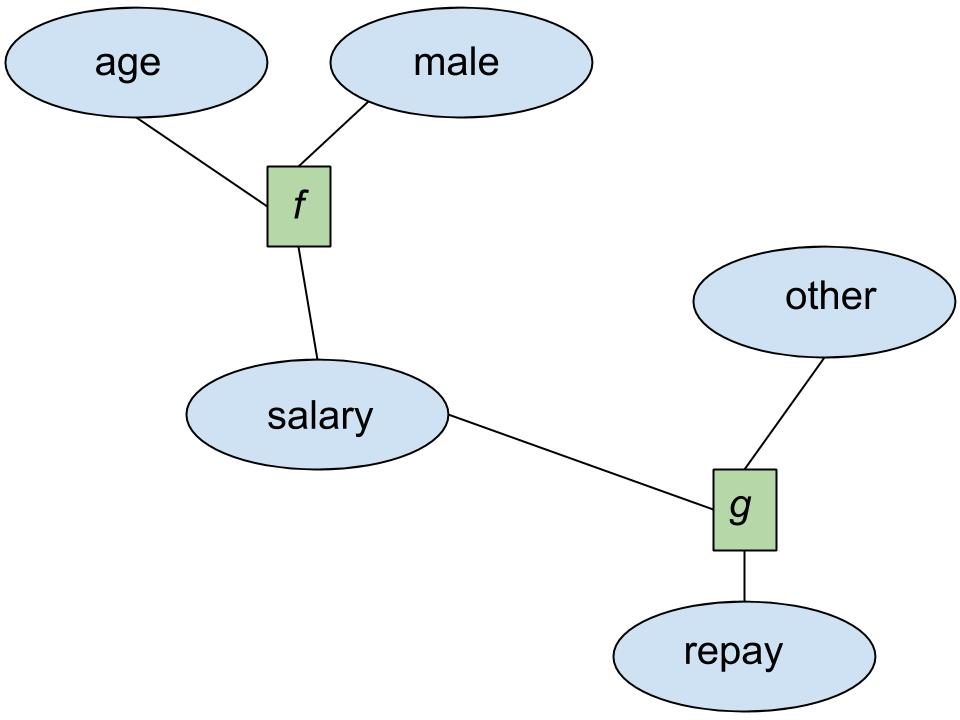
\includegraphics[width=0.33\textwidth]{fg}
}
\end{figure}

\subsection{Structure}
The structure of a factor graph is an undirected, bipartite graph.
A bipartite graph is one in which you can divide all of its nodes into two disjoint subsets such that every edge in the graph connects
a node in one subset to a node in the other subset. Figure~\ref{fig:f1}(c) is an example of a factor graph.
In this example, the set of square nodes and the set of circle nodes are disjoint because the circles only connect to squares and the squares only connect to circles.

\subsection{Parameters}
The parameters of a factor graph are called ``factors" or ``node potentials", which are represented by the square nodes in figure~\ref{fig:f1}(c). 
Each node potential is a real-valued function, and the arguments to that function are the neighbors of that potential. 
For example, the neighbors of the $f$ node in figure~\ref{fig:f1}(c) are \textit{age}, \textit{male}, and \textit{salary}, 
and thus the node potential of $f$ is a function of  \textit{age}, \textit{male}, and \textit{salary}.

The tables (a) and (b) in figure~\ref{fig:f1} represent possible functions for potentials $f$ and $g$, respectively. 
We can represent a potential using a table as long as the arguments are discrete.
To do this, we add a tuple to our table for each of the possible values that the arguments can take.
The tuples determine the value of $f$ for a specific set of argument values.
For example, to determine the value of function $f$ for $age=T$ (i.e., older), $male=F$ (i.e., female), and $salary=F$ (i.e., low salary), we can look up these argument values in table~\ref{fig:f1}(a) and see that the $f$ has the value 1.

\subsection{Probabilities}
The structure and parameters determine the probability distribution. The overall probability can be found by multiplying together all of the factors and then dividing by a normalizing constant:
\begin{equation*}
P(x)=\frac{1}{Z}\prod_{factors\,k}\Phi_k(x_{arg(k)})
\end{equation*}
where $\Phi_k$ is the factor, $X_{arg(k)}$ are the argument values of the factors (i.e., the values of the factor's neighbors in the graph), and $Z$ is the normalizing constant.

For example, the probability of figure~\ref{fig:f1}(c) can be written as:
\begin{equation*}
\begin{split}
P(x) & =\frac{1}{Z}\prod_{i\epsilon\{f,g\}}\Phi_i(x_{arg(i)}) \\
& =\frac{1}{Z}\Phi_f(X_{arg(f)})\Phi_g(x_{arg(g)}) \\
& =\frac{1}{Z}\Phi_f(a,m,s)\Phi_g(s,o,r)
\end{split}
\end{equation*}

Note that Bayes net equation does not have a normalizing constant, $Z$.
The addition of $Z$ results in a number of differences between factor graphs and Bayes nets.
One example of a difference is that $Z$ increases the computational complexity.
In general, computing $Z$ is non-trivial and takes exponential time because it is equal to the sum 
the values of the product of potentials over all possible assignments.
Later, we will study more efficient ways to compute $Z$ that work for certain cases.

\section{Markov Random Field}
\begin{figure}[h]
\caption{Markov Random Field (MRF)}
\label{fig:f3}
\centering
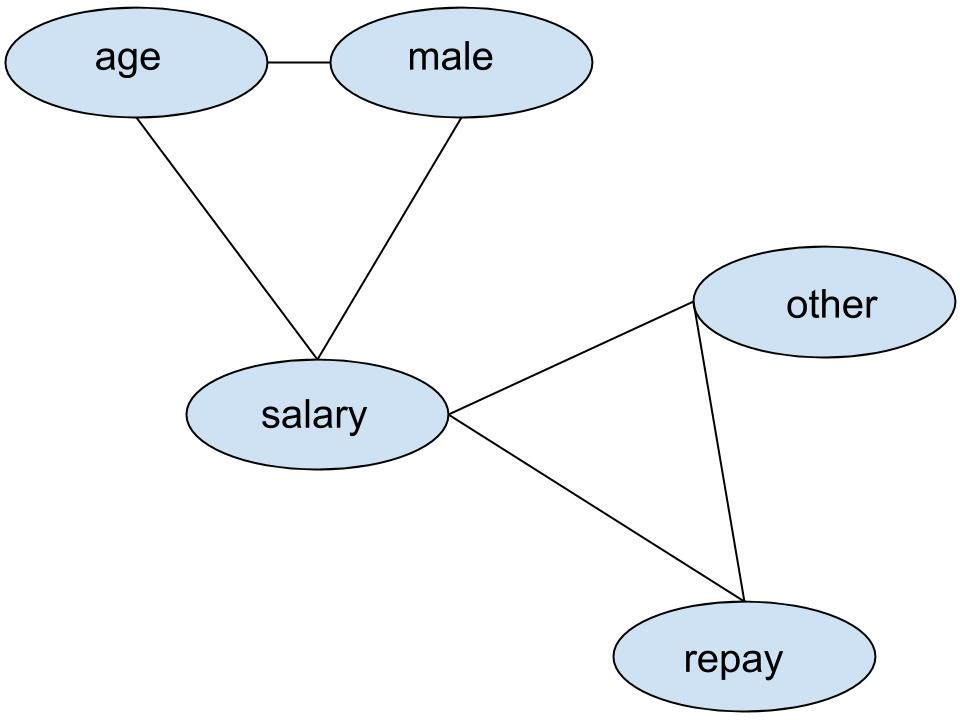
\includegraphics[width=0.4\textwidth]{MRF}
\end{figure}

Another type of graphical model is a Markov random field (MRF).
Again, graphical models are given by a structure and a set of parameters.
The structure in a MRF is simply an undirected graph, (note that this particular graphical model can have cycles).

A clique in a graph is a set of nodes that are connected in all possible ways with one another 
(e.g., a three-clique is a triangle, a four-clique is a square with a cross in the center).
The parameters in a MRF are cliques.
For every clique, there is a factor (or potential), just like the factor in a factor graph.
In fact, we can think of the MRF being an alternate notation for a factor graph 
with the exception that
 instead of having a clique in a factor graph, you have an explicit notation for where all of the factors are.

Figure~\ref{fig:f3} shows the factor graph from figure~\ref{fig:f1}(c) drawn as a MRF.
This graph is created by replacing factors $f$ and $g$ with 3-cliques.

\section{Factor Graphs and MRF: Testing for Conditional Independence}
Like Bayes nets, factor graphs and MRFs can also be tested for conditional independence.
To perform this test, you first delete all of the observed nodes from the graph 
(along with their outgoing edges) and then check for a path. 
\begin{figure}[h]
\caption{}
\label{fig:f2}
\centering
\subfloat[Example 1]{ 
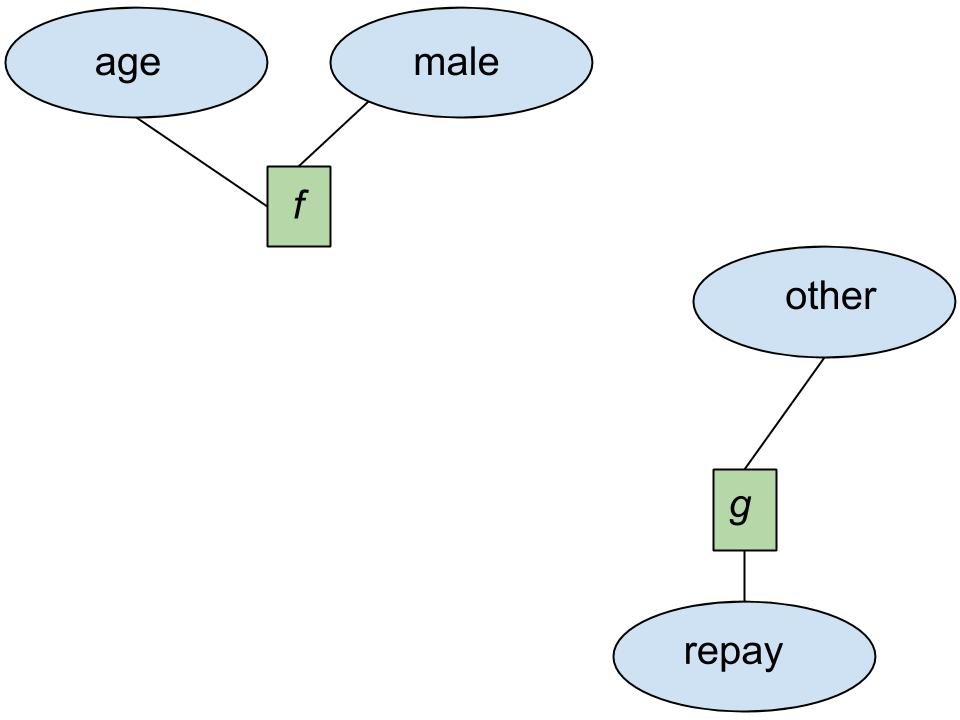
\includegraphics[width=0.4\textwidth]{fg_ex1}
}
\hfill
\subfloat[Example 2]{ 
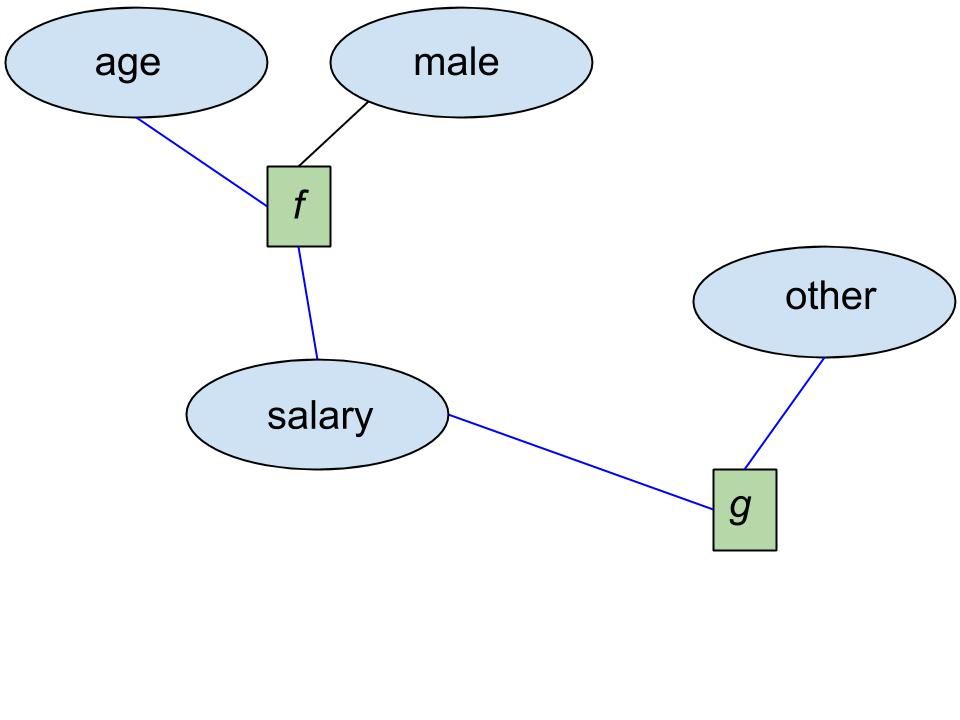
\includegraphics[width=0.4\textwidth]{fg_ex2}
}
\end{figure}

\textbf{Example 1: is \textit{age} independent of \textit{repay} given \textit{salary}?}
Removing $salary$ and its outgoing edges from the graph splits the graph into two.
Since there is no path between $age$ and $repay$, it is true that $age$ is independent of $repay$ given $salary$.

\textbf{Example 2: is \textit{age} independent of \textit{other} given \textit{repay}?}
After removing $repay$ and it's outgoing edges from the graph, there is still a path from $age$ to $other$,
so $age$ is not independent of $other$ given $repay$.

FIGURES XXX and~\ref{fig:f1}(c) show the same probability distribution represented by a Bayes net and a factor graph, respectively.
If we ask whether age and male are independent in the Bayes net representation,
d-separation will determine that they are independent since there is no active path between them. If we ask whether age and
male are independent in our factor graph, the graphical test will determine that they are not independent
since there is a path between them.

It may seem strange that these representations have different sets of conditional independences for the same
distribution.
But, remember how in graphical models some of the conditional independences are determined
by the graphical structure, and others depend on the parameters (e.g., conditional probability tables of the Bayes net
or the factors in factor graph).
So, in our example, by going back and forth between the two representations, we have changed the set of 
conditional independences that are determined by the graphical model's structure versus the ones that are accidental.

Notice that the factor graph has a smaller set of conditional independences.
In general, if you take a Bayes net and turn it into a factor graph that represents the same distribution,
you'll have fewer (non-accidental) conditional independences in the factor graph.
This is another subtle difference between the two models.
Generally, if you have a distribution, its actual conditional 
independence relationships might be captured better by one model than another.
This is one reason you might to choose one particular model over another.

\section{Converting Between Bayes Net, Factor Graph, and MRF Representations}
Bayes nets, factor graphs, and MRFs can represent every probability distribution in some form.
This means that it's possible to convert among the different representations, and converting between these representations is relatively easy.

Unfortunately, you can lose some information about independences during the conversion process because
when you make the conversion, independences that were explicit can become accidental.
Still, there are many cases where being able to convert between these models is advantageous.
For example, if you have software that only works for factor graphs but you are given a Bayes net 
representation, then having the ability to convert between these models would be beneficial.

\begin{figure}[h]
\caption{Converting between Bayes Net, Factor Graph, and MRF representations}
\label{fig:f4}
\centering
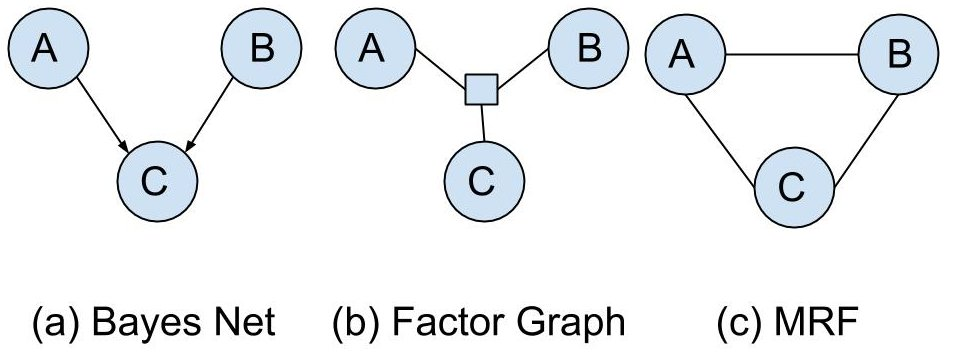
\includegraphics[width=0.6\textwidth]{conv}
\end{figure}

\begin{enumerate}
\item \textbf{Converting from a Bayes net to a factor graph:} \\
If you have a Bayes net, the probability distribution is already represented as a product of factors.
Each factor happens to be a conditional probability table, but you can simply treat each of these tables as factors.
For example, to convert the Bayes net graph with $P(C|A,B)$ in figure~\ref{fig:f4}(a), we turn it into $\Phi(A,B,C)$ and make
a factor graph that has a factor connecting $A$, $B$, and $C$ (shown in figure~\ref{fig:f4}(b)).

\item \textbf{Converting from a factor graph to a MRF} \\
A factor graph can be converted into a MRF by taking each factor and drawing a clique on it. 
In our example, the factor in the is connected to three arguments.
To convert this factor graph to a MRF, we remove the factor and draw a 3-clique to reconnect the arguments.
Figure~\ref{fig:f4}(c) shows the resulting MRF.

Converting from a factor graph to a MRF may introduce extra cliques.
We supply any extra cliques a potential that is always 1 so that our probability calculations remain unchanged.

\item \textbf{Converting a MRF to a factor graph} \\
To convert a MRF to a factor graph, we find each clique in the MRF and replace it by a factor.
The potential of the particular clique we replaced becomes the potential of the factor that replaced it.

\item \textbf{Converting a MRF to a Bayes net} \\
Converting from a MRF back to a Bayes is the most difficult method out of the four described in this section
because it requires more computation.
There's an expensive way and a cheap way to do this.

\begin{enumerate}
\item \textit{The expensive way:} \\
First, we pick a root from the MRF graph and direct the edges away from the root in a way that does not introduce cycles.
Then we can run Bayes net inference and use the results as our conditional probability table.
This method is expensive because we must run Bayes inference to find every conditional probability table.

\begin{figure}[h]
\caption{Converting from MRF back to Bayes net the expensive way}
\label{fig:f5}
\centering
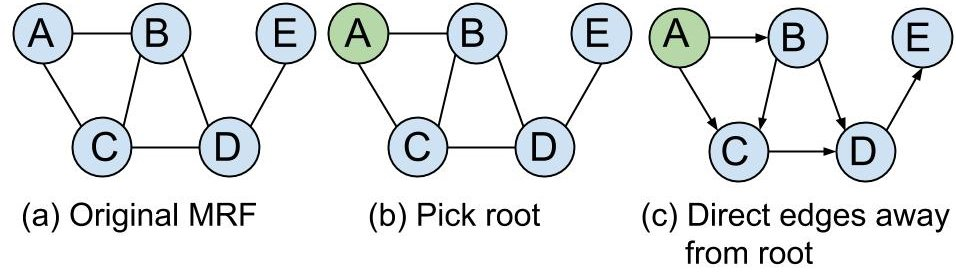
\includegraphics[width=0.6\textwidth]{exp}
\end{figure}

\item \textit{The cheap way}: \\
To do the cheap conversion, we add an observed common child for each factor.
There is always a way to set the conditional probability table of $A,B,C$ and to pick an observation for $Z$ 
(e.g., we can observe Z to be true) such that we can replicate the particular factor.
A disadvantage of this approach is that adding in extra children increases the size of the graph.
\end{enumerate}

\begin{figure}[h]
\caption{Converting from MRF back to Bayes net the cheap way}
\label{fig:f6}
\centering
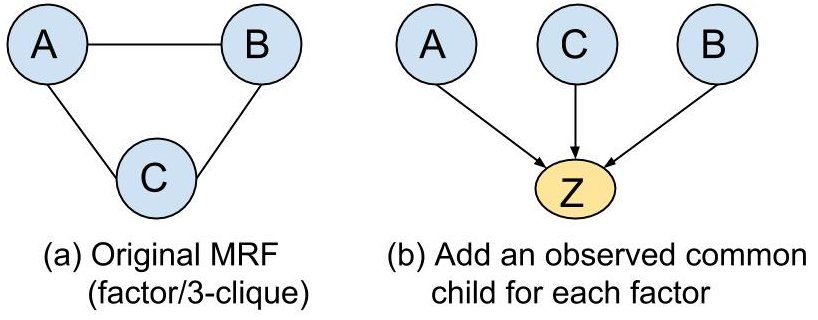
\includegraphics[width=0.5\textwidth]{cheap}
\end{figure}

\end{enumerate}

\section{Choosing a Graphical Model}
Some distributions have a better representation in one graphical model than another. For example, one model
may capture more explicit conditional independences than others.
Some operations are easier in one type of graph than another.
For example, structure learning is easier in factor graphs than in Bayes nets
whereas some inferences are much cheaper in Bayes nets than factor graphs because 
you can avoid computing the normalizing constant.

\end{document}

